\chapter{Capacidades de PCL: Objetivos y herramientas}
\section{Capacidades de PCL}
\subsubsection{Módulo io}
Uno de los módulos más importantes es el que se encarga de la lectura y escritura de nubes de puntos, es decir, el módulo IO del inglés input/output que se traduce como entrada/salida. Es por tanto esta librería capaz de interpretar la información otorgada por diferentes tipos de sensores así como de generar archivos que contienen nubes de puntos manipuladas por el resto de módulos.
Existen varios tipos de formatos bajo los que almacenar una nube puntos.

PCL ha creado el formato PCD, del inglés Point Cloud Data, es decir datos de nube de puntos. No se trata de un formato revolucionario sino más bien de una forma de complementar a los ya existentes que debido a los propósitos para los que se han creado u otras razones, no soportan algunas de las características relacionas con al procesamiento de nubes de puntos de n dimensiones. Además sufren de deficiencias en ciertos campos de computación debido a que fueron creados para fines diferentes, en diferentes épocas y en ocasiones mucho antes de la invención de los sensores y algoritmos hoy presentes.

Por lo tanto, el formato PCD no es único ni trata de reemplazar a los que ya están presentes creados por comunidades de computación gráfica y geométrica que en concreto sirven para describir polígonos arbitrarios y nubes de puntos obtenidas con escáneres láser. Por ejemplo se tienen formatos como los siguientes:


PLY - Formato de ficheros para polígonos creado por Turk et al de la universidad de Stanford
STL - Un formato nativo para software CAD de estereolitografía creado por 3D systems 
OBJ - Un software de definición geométrica creado por Wavefront Technologies 
X3D - Un formato basado en la norma ISO de XML para la representación de gráficos en 3d para computadoras 

Puesto que a partir de ahora se va a utilizar el formato PCD, se va a explicar con mayor profundidad cada una de sus partes.

Un fichero PCD dispone de dos partes diferenciadas, encabezamiento y los puntos como tal.

El encabezamiento se encarga de identificar y declarar las propiedades de la nube de puntos almacenados en el fichero y debe estar codificado en ASCII lo que implica que cada entrada en este formato está delimitada de las demás usando saltos de línea.

Las características especificadas en el encabezamiento son las siguientes:

\begin{itemize}
\item VERSION:
Este campo especifica la versión del formato PCD

\item FIELDS
Traducido como "campos" indica el nombre de cada dimensión o campo existente en la nube de puntos como por ejemplo color, coordenadas XYZ o normales a la superficie.

\item SIZE 
Este campo indica el tamaño en bytes y en el mismo orden de cada campo declarado por FIELDS 

\item TYPE
Representa el tipo de dato de cada campo con un carácter. 
I: Tipos con signo como int8 que equivale a un char, int16 que equivale a un short y int32 que equivale a un int
U: Tipos sin signo como uint8, uint16 y uint32, los tipos análogos al caso anterior pero sin signo
F: Representa todos los tipos flotantes

\item COUNT 
Indica cuántos elementos tiene cada campo previamente declarado en FIELDS. Por defecto toma el valor de 1.

\item WIDTH
Representa el ancho de la nube de puntos teniendo este concepto dos significados para lo cual hay que entender cómo se puede interpretar una nube de puntos. Por una parte, las nubes de puntos desorganizadas pueden verse como un vector de n elementos donde n es el ancho de la nube de puntos, es decir, se trata de una matriz de una fila y n columnas donde n es el ancho. Por otra parte, se puede definir de manera matricial con m filas y n columnas siendo ahora m el número de puntos presentes en cada columna y lo que define una nube de puntos organizada.

\item HEIGHT
No es nada más que el número de filas de la nube de puntos en su representación matricial explicada en el apartado anterior o bien el numero total de puntos de una nube representada como una matriz de m filas y una columna siendo en este caso m el campo tratado en este apartado.

\item VIEWPOINT
Especifica la posición del punto de vista desde el que el sensor adquirió la nube de puntos. Se indica como una traslación tx, ty, tz así como con un cuaternio qw, qx, qy, qz con un valor por defecto de 0 0 0 1 0 0 0 respectivamente.

\item POINTS
Indica el número total de puntos en la nube. Puesto que se trata de información redundante dados los campos previamente descritos, se espera que éste sea eliminado en un futuro.

\item DATA
Es el tipo de dato con el que se ha generado el fichero PCD siendo dos formatos los soportados, ascii y binary. El formato ascii obliga a que cada punto se escriba en una nueva línea, mientras que en el formato binary, la información presente en el fichero es una copia en memoria de la nube de puntos como vector de forma que se incrementa la velocidad de lectura y escritura
\end{itemize}

Queda el encabezamiento entonces con la siguiente estructura:

VERSION\\
FIELDS\\
SIZE\\
TYPE\\
COUNT\\
WIDTH\\
HEIGHT\\
VIEWPOINT\\
POINTS\\
DATA\\

Como se ha mencionado previamente, cada punto se introduce después del encabezado en una línea nueva indicando, separados por espacios, el valor de cada campo. Como ejemplo de nube de puntos en formato PCD se tiene lo siguiente:

VERSION .7\\
FIELDS x y z rgb\\
SIZE 4 4 4 4\\
TYPE F F F F\\
COUNT 1 1 1 1\\
WIDTH 213\\
HEIGHT 1\\
VIEWPOINT 0 0 0 1 0 0 0\\
POINTS 5\\
DATA ascii\\
0.93773 0.33763 0 4.2108e+06\\
0.90805 0.35641 0 4.2108e+06\\
0.81915 0.32 0 4.2108e+06\\
0.97192 0.278 0 4.2108e+06\\
0.944 0.29474 0 4.2108e+06\\

\subsubsection{Módulo registration}
A parte del módulo básico de lectura y escritura, PCL dispone de un importante módulo llamado registration que se encarga del alineamiento de nubes de puntos independientes para ser fusionadas en una sola de forma coherente y así poder proceder con futuras operaciones sobre la nube resultante como reconocimiento de objetos o reconstrucción de superficie.

Normalmente, las nubes de puntos son adquiridas desde diferentes puntos de vista o incluso con varios sensores por lo que es fundamental encontrar las posiciones y orientaciones relativas de cada nube respecto a un sistema de coordenadas global de manera que las partes que son idénticas se solapen perfectamente.

La manera de alinear las nubes de puntos se basa en encontrar correspondencias entre las mismas, es decir, puntos semejantes, y entonces estimar transformaciones que trasladan y rotan las nubes de entrada para que queden alineadas en una sola.

Se suele tomar un modelo o nube de entrada como modelo o referencia de forma que sean las demás nubes a las que se les aplica la transformación adecuada para que se parezcan al modelo. 

De esta forma, dadas dos ...

Se trata de una fácil tarea si se conocen de antemano las correspondencias entre las nubes de entrada. Esto implica que un conjunto de puntos pertenecientes a una nube A ha de coincidir con su conjunto de puntos equivalente de una nube B. Además, si las correspondencias y por tanto el alineamiento, son perfectos entonces se tiene una solución cerrada

PCL contiene algoritmos que permiten detectar diferentes tipos de correspondencias entre nubes así como métodos para desechar las que no resultan útiles y estimar transformaciones robustas.

Un sencillo ejemplo visual de lo que puede hacer este módulo se muestra en la figura \ref{fig:registration_bunny} donde se tienen dos nubes de puntos muy parecidas que se fusionan en una sola. 


\begin{figure}
\centering
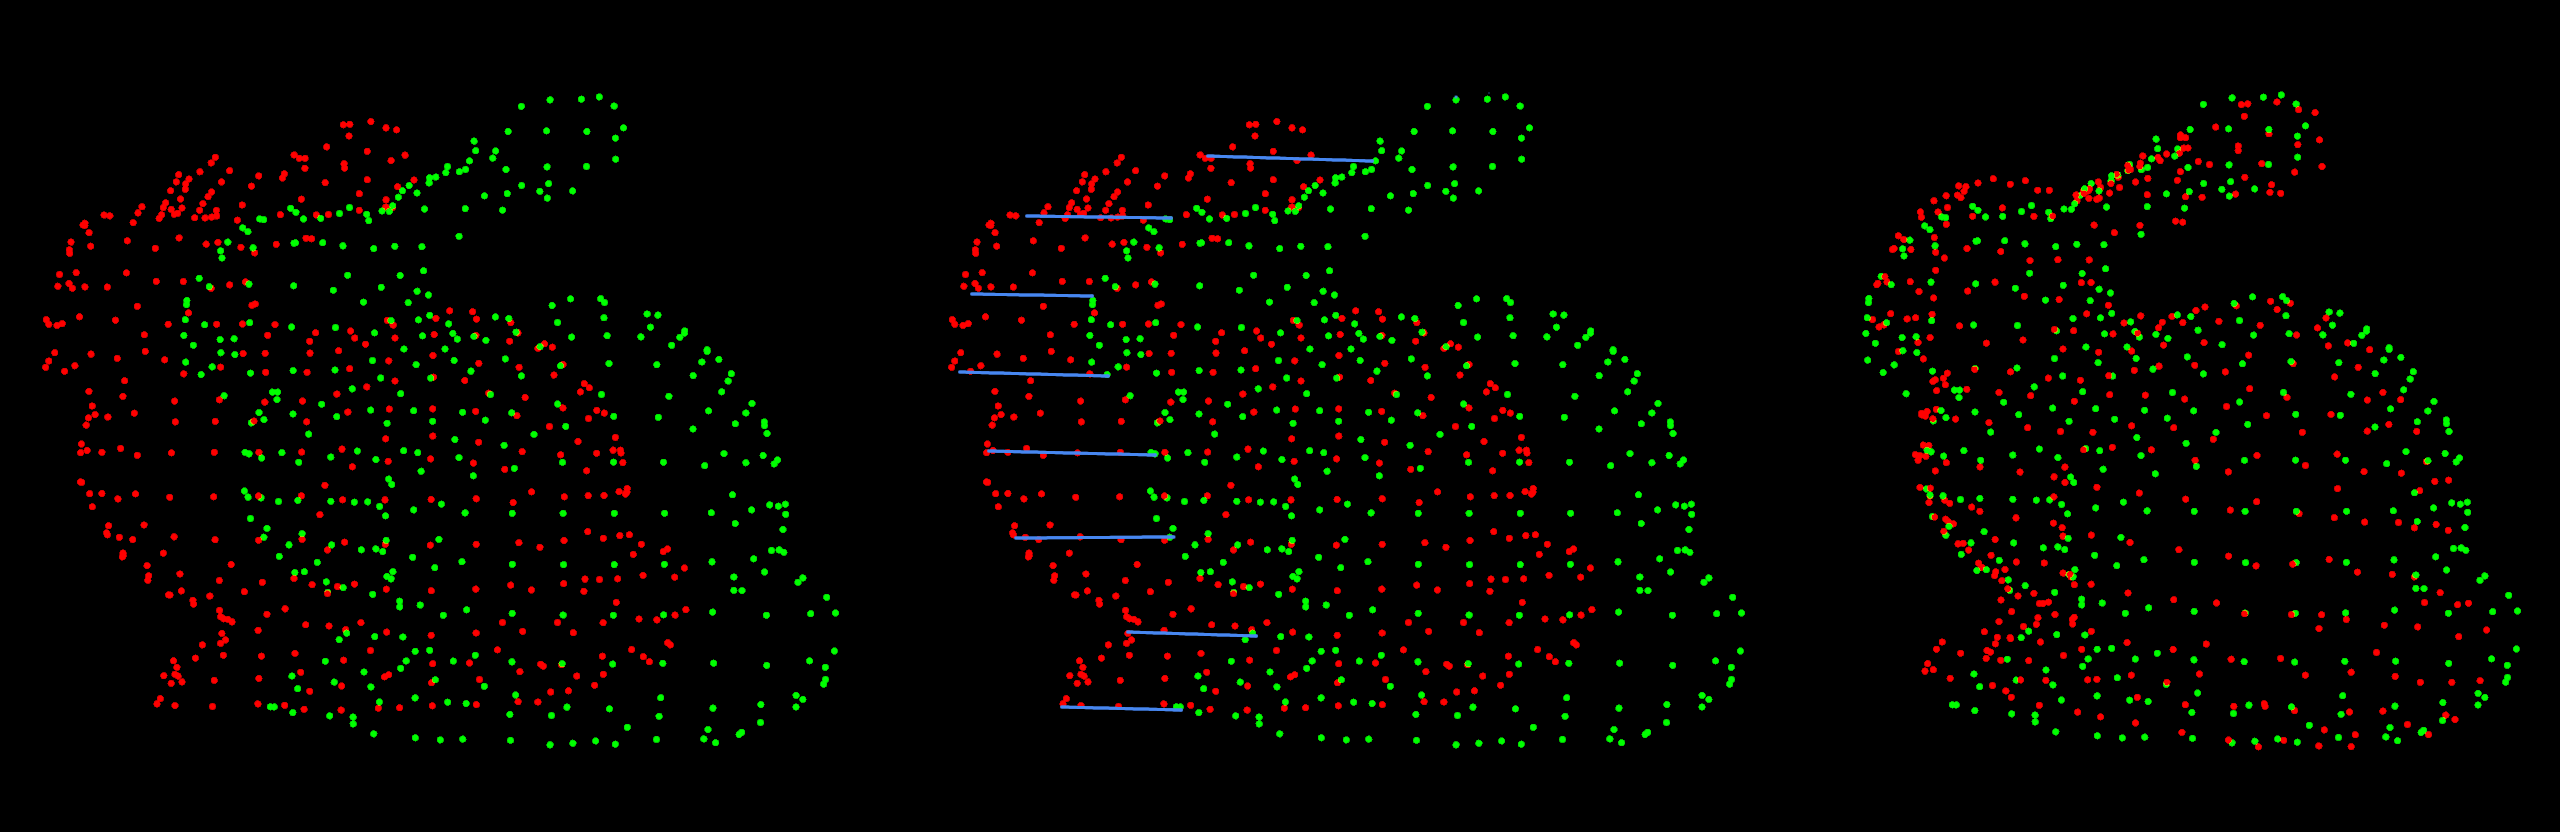
\includegraphics[scale=0.15]{registration_bunny}
\caption{Ejemplo de alineamiento de dos nubes de puntos.}\label{fig:registration_bunny}
\end{figure}



Para conocer en mayor detalle el proceso de alineamiento, se muestra en la figura \ref{fig:registration_flow} el conjunto de pasos que se siguen desde que se indican las nubes de entrada hasta que se obtiene la fusión de las mismas.
\begin{figure}
\centering
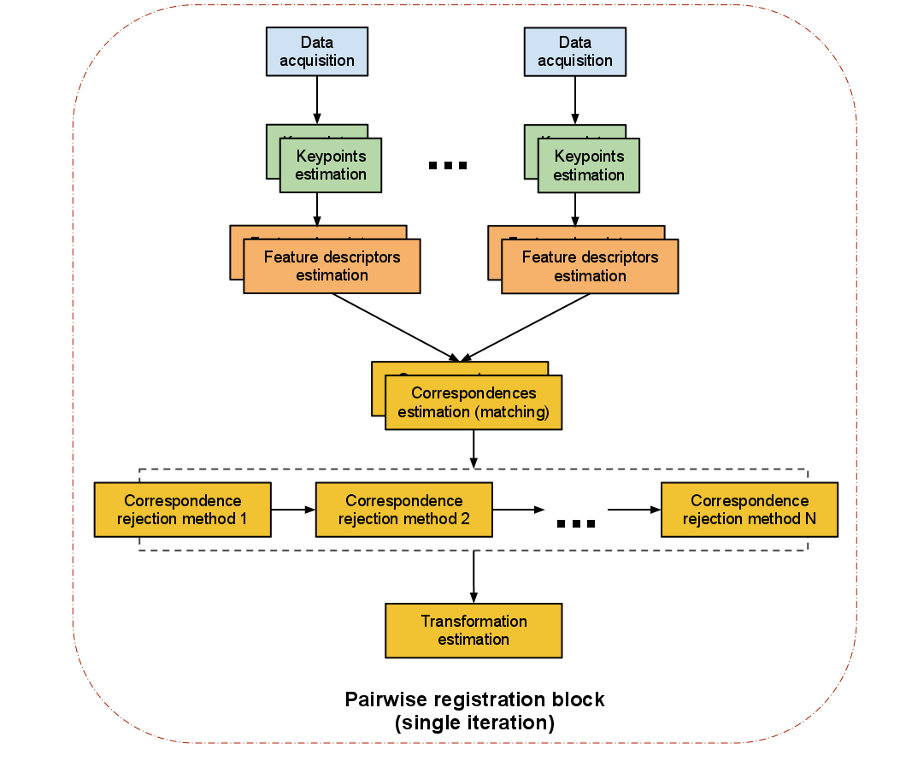
\includegraphics[scale=0.5]{registration_flow}
\caption{Procedimiento completo para llevar a cabo el alineamiento de nubes de puntos.}\label{fig:registration_flow}
\end{figure}


Dadas dos o más nubes de puntos como entrada, el primer paso implica extraer keypoints o puntos clave de cada una de ellas. Por keypoint, punto clave o punto de interés se entiende como un punto de la nube que representa características especiales de la misma tal como esquinas o bordes. Por tanto, las principales características de un keypoint pueden resumirse en los siguientes puntos:

%https://en.wikipedia.org/wiki/Interest_point_detection

\begin{itemize}
\item[•] Tiene una clara definición matemática
\item[•] Tiene una clara definición de su posición en el espacio
\item[•] El entorno local alrededor del keypoint es rico en información característica de la nube de modo que el uso del keypoint simplifica el uso de la nube
\item[•] Es estable ante perturbaciones locales y globales tal y como cambios de iluminación y brillo de modo que las operaciones aplicadas sobre estos puntos tengan elevada repetibilidad
\item[•] De forma opcional, el keypoint puede incluir un atributo de escala para poder aplicar operaciones sobre keypoints obtenidos de imágenes reales así como poder tolerar cambios de escala
\end{itemize}

Por ejemplo, las esquinas detectadas en una nube de puntos o imagen pueden considerarse puntos clave pues muestran información característica sobre las delimitaciones del objeto detectado tal y como se aprecia en la figura \ref{fig:corner_detection}

\begin{figure}
\centering
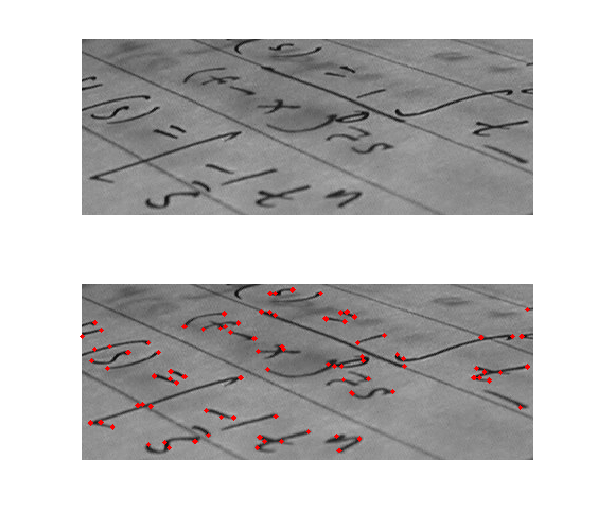
\includegraphics[scale=0.5]{corner_detection}
\caption{Ejemplo de detección de puntos clave en forma de esquinas.}\label{fig:corner_detection}
\end{figure}

Obtener correctamente los keypoints es de vital importancia ya que intentar alinear dos nubes considerando todos y cada uno de sus puntos puede suponer una carga computacional inconcebible para el caso de nubes de cientos de miles o incluso millones de puntos. 

A continuación se procede a la estimación de los feature descriptors, es decir, los vectores donde se almacenan las características de la nube entorno a cada keypoint para poder compararlos entre sí. Por ejemplo se puede tener un vector que contiene normales a la superficie en cada keypoint o bien información sobre el brillo o luminosidad.


Una vez que se dispone de dos o más vectores de características, cada uno de una nube de puntos diferente, hay que encontrar la información equivalente entre vectores, es decir, las características de las nubes que pueden solaparse ya que son muy parecidas o idénticas. Dependiendo del tipo de característica que se quiera alinear o unificar existen diferentes métodos para encontrar correspondencias:


Para hacer coincidir puntos utilizando solamente sus coordenadas XYZ existen métodos tanto para nubes organizadas como desorganizadas:

brute force matching,
kd-tree nearest neighbor search (FLANN),
searching in the image space of organized data, and
searching in the index space of organized data.

Para la coincidencia de características diferentes a la posición de los puntos se tienen los siguientes métodos: 


brute force matching and
kd-tree nearest neighbor search (FLANN).
Direct correspondence estimation (default) searches for correspondences in cloud B for every point in cloud A .
“Reciprocal” correspondence estimation searches for correspondences from cloud A to cloud B, and from B to A and only use the intersection.



\section{Objetivos del TFG}
Generar un programa capaz de obtener keypoints a partir de una nube de puntos
Croscompilar usando las herramientas de xilinx 
Enviar ejecutable a la placa y ejecutar el programa
(optimización)

%http://pointclouds.org/
\section{Herramientas necesarias para desarrollar el trabajo}
\subsection{Herramientas hardware}
\subsection{Herramientas software}
